\documentclass[a4paper, 11pt]{article}
\usepackage{fancyhdr}
\usepackage{fullpage}
\usepackage{times}
%\usepackage[french]{babel}
\usepackage{sverb}
%\usepackage[T1]{fontenc}
\usepackage{proof}
\usepackage{amssymb}
\usepackage{amsmath}
\usepackage{stmaryrd}
\usepackage{amscd}
\usepackage{marvosym}
\usepackage{eurosym}
\usepackage{alltt}
\usepackage{url}

\usepackage{paralist}
\usepackage{pgf}
\usepackage{multicol}

\usepackage{ae,lmodern} % ou seulement l'un, ou l'autre, ou times etc.
\usepackage[francais]{babel}
\usepackage[utf8]{inputenc}
\usepackage[T1]{fontenc}

\usepackage{listings}

%\usepackage[utf8]{inputenc}
%\usepackage[latin1]{inputenc}

\pagestyle{fancy}
\setlength\headheight{10mm}
\setlength\headsep{5pt}

\lhead{IESE5}
\chead{Architecture des processeurs - S9}
\rhead{\pgfimage[height=.7cm]{logo_polytech}}

\lfoot{H.P. Charles \& César Fuguet \& F. Rousseau}
\rfoot{Page : \thepage}
\cfoot{} 

\lstset{language=C,
  basicstyle=\ttfamily,
  commentstyle=\it,
  extendedchars=false,
  texcl=true,
}
\newtheorem{question}{Question}

\date{\relax}
\title{\Large{\textbf{Examen 1h30\\Programmation RISCV\\Performance et synchronisation\\Documents et calculatrice autorisés}}}
\author{}


\newcommand{\extitle}[2]{\textbf{Exercice #1~:}~{\large\textbf{#2}}}

\begin{document}


\maketitle
\thispagestyle{fancy}

%------------------------------------------------------------------------------------


L'examen est composé de 2 exercices chacun noté sur 10 points, \textbf{à rédiger sur des feuilles différentes}.


%\expartie{1}{Efficacité de la mémoire cache}
\section{Etude d'un programme en langage d'assemblage RISC-V}

Vous venez de récupérer le bout de programme en langage d'assemblage RISC-V suivant :

\begin{lstlisting}

800000e0 <inconnu>:
800000e0:    ff410113     addi  sp,sp,-12
800000e4:    00112423     sw    ra,8(sp)
800000e8:    00a12223     sw    a0,4(sp)
800000ec:    00b12023     sw    a1,0(sp)
800000f0:    00058c63     beq   a1, <fin1>
800000f4:    ????????     addi  a1,a1,-1
800000f8:    ????????     jal   ra, <inconnu>
800000fc:    ????????     lw    a2,4(sp)
80000100:    02c50533     mul   a0,a0,a2
80000104:    0080006f     jal   zero, <fin2>

80000108 <fin1>:
80000108:    00100513     addi  a0,zero,1

8000010c <fin2>:
8000010c:    00812083     lw    ra,8(sp)
80000110:    00012583     lw    a1,0(sp)
80000114:    00c10113     addi  sp,sp,12
80000118:    00008067     jalr  zero,0(ra)

\end{lstlisting}

Il s'agit d'un fichier desassemblé, qui fait apparaître sur une ligne soit
l'adresse et l'étiquette, soit l'adresse, le codage binaire de l'instruction et l'instruction désassemblée.
Par exemple, à l'adresse 0x800000e0, l'instruction addi sp,sp,-12 est codée en binaire par 0xff410113.
L'adresse 0x800000e0 correspond à l'étiquette <inconnu>, nom de la fonction à découvrir.

On cherche en effet à retrouver l'équivalent en C de cette fonction, et sa fonctionnalité !


\begin{question}
Vous avez noté la série de ???????? qui indique que le codage binaire de 3 instructions a disparu !
En utilisant en annexe le codage du jeu d'instructions et les numéros de registres, donnez le codage binaire de ces 3 instructions.
% correction
% 800000f4:    fff58593     addi  a1,a1,-1
% 800000f8:    fe9ff0ef     jal   ra, <inconnu>
% 800000fc:    00412603     lw    a2,4(sp)
\end{question}


Dans le \textit{main}, on trouve l'appel à la fonction <inconnu> à l'adresse 0x80000080.

\begin{lstlisting}
80000078 <main>:
80000078:    00300513     addi  a0,zero,3
8000007c:    00400593     addi  a1,zero,4
80000080:    060000ef     jal   ra,<inconnu>
...
\end{lstlisting}

\begin{question}
A l’entrée dans la fonction <inconnu>, on observe que sp = 0x80110290. Indiquer les adresses mémoire et le contenu de ces adresses après l'exécution des 4 premières instructions de la fonction <inconnu>.
% 0x80110284:	0x00000004	0x00000003	0x80000084
\end{question}


\begin{question}
Vous avez certainement noté que la fonction <inconnu> contient un appel à elle même. Il s'agit donc d'une fonction récursive.
Retrouvez la condition d'arrêt de la fonction, c'est à dire la condition qui stoppe les appels récursifs. Comment l'écririez vous en langage C ?
%  int inconnu (int x, int n)
% {
% if (n == 0)
%       return 1;
\end{question}


\begin{question}
On souhaite dessiner la pile qui correspond à l’exécution de la fonction <inconnu>, en commençant à son appel depuis le main et jusqu'à la condition d'arrêt. 
Indiquer les valeurs et les adresses de façon précise. Indiquer ind quand le contenu de la pile n’est pas précisé.

% (gdb) x /12x $sp
% 0x80110260:	0x00000001	0x00000003	0x800000fc	0x00000002
% 0x80110270:	0x00000003	0x800000fc	0x00000003	0x00000003
% 0x80110280:	0x800000fc	0x00000004	0x00000003	0x80000084
% (gdb) 

\end{question}


\begin{question}
Retrouvez l'équivalent en langage C de la fonction <inconnu>. Pour cela, on pourra retrouver le calcul effectué après le retour de l'appel récursif.

% /* Prototype de la fonction PuissanceEntiere en récursif */
% unsigned int puis_rec(unsigned int x, unsigned int n)
% {
% if (n == 0)
%       return 1;
% return x × puis_rec(x, n - 1);
% }

\end{question}

\begin{question}
Quelle est la fonctionnalité de la fonction ?
% Calcul de x à la puissance n
\end{question}


 \newpage

\section{Structure de cache et programmation}

Le nouveau processeur P650 de la société SiFive est un multiprocesseur 
RISCV contenant plusieurs cœurs RISCV 64 bits. Il contient 16 cœurs, 16 Mo 
de cache L3, 256 Ko de cache L2 et 64 Ko de cache L1 divisé en 32 Ko de cache 
instructions et 32 Ko de cache données. Comme sur beaucoup de processeurs 
les adresses utilisées indiquent une adresse d'octet.

Données du problème :
\begin{itemize}
    \item Dans la suite de cet exercice on s'intéressera uniquement au cache L1 données de 32 Ko. On sait que ce cache est associatif à 4 voies.
    \item On supposera que les valeurs des  adresses réellement utilisées sont sur 44 bits.
    \item On supposera que les lignes de caches contiennent 8 mots de 64 bits.
\end{itemize}


\begin{center}
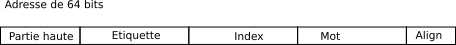
\includegraphics[width=.9\textwidth]{CacheAssociatif.png}
\vspace{2ex}
\end{center}

\begin{question} Une adresse mémoire arrivant vers le cache sera divisée en plusieurs champs indiqués dans la figure précédente. Quelles sont les caractéristiques (longueur et valeur) des champs \textbf{Align} et \textbf{Partie haute}. Pourquoi ?
\end{question}
% Align : contient 3 zeros en partie droite (les mots de 64 bits sont alignés
% sur des adresses multiple de 64)
% Partie haute n'est pas utilisé : seuls les 44 bits sont utilisés

\begin{question} Le constructeur indique que la partie donnée du cache L1 fait 32 Ko 
associatif à 4 voies. Les lignes de caches contiennent 8 mots de 64 bits. 
Quelle est la taille (en octet) d'une ligne ? Quelles sont les largeurs 
des différents champs \textbf{Etiquette}, \textbf{Index} et \textbf{Mot} ? 
Indiquez votre raisonnement !
\end{question}
% Mot = 3 bits pour sélectionner 1 mot parmis 8
% TailleLigne = 1 ligne = 8 mots x 8 octets = 64 octet
% 32 Ko / 4 = 8Ko par voies TailleVoie
% NLigne = TailleVoie / Taille Ligne = 8192 / 64 = 128 lignes = Index de 7 bits
% Etiquette = 44 - (3 + 3 + 7) = 31 bits


\begin{question}
Quelle est la taille totale du cache en bits ? (la taille des données, des tags, bit de validité 
et des différentes voies)
\end{question}

\begin{question}
On charge une donnée de 64 bits dont l'adresse est 0x00000E935B87E298. 
Quel est le numéro de la ligne
de cache dans laquelle cette donnée sera stockée ?
\end{question}
% 0xE935B87E298 = 1110100100110101101110000111111 0001010 011 000
%                 Etiquette                       Index   Mot
% Index = 10

\begin{question}
Soit un programme, en C, utilisant un tableau à une dimension contenant 20 mots de 64 bits.
Le programme doit faire la somme des 20 valeurs. En supposant qu'un accès à une donnée permet
de remplir une ligne entière de cache, combien de défaut de cache ce programme va provoquer ?
Pourquoi ?
\end{question}
% \section{Synchronisation RISCV}

\newpage

\begin{center}
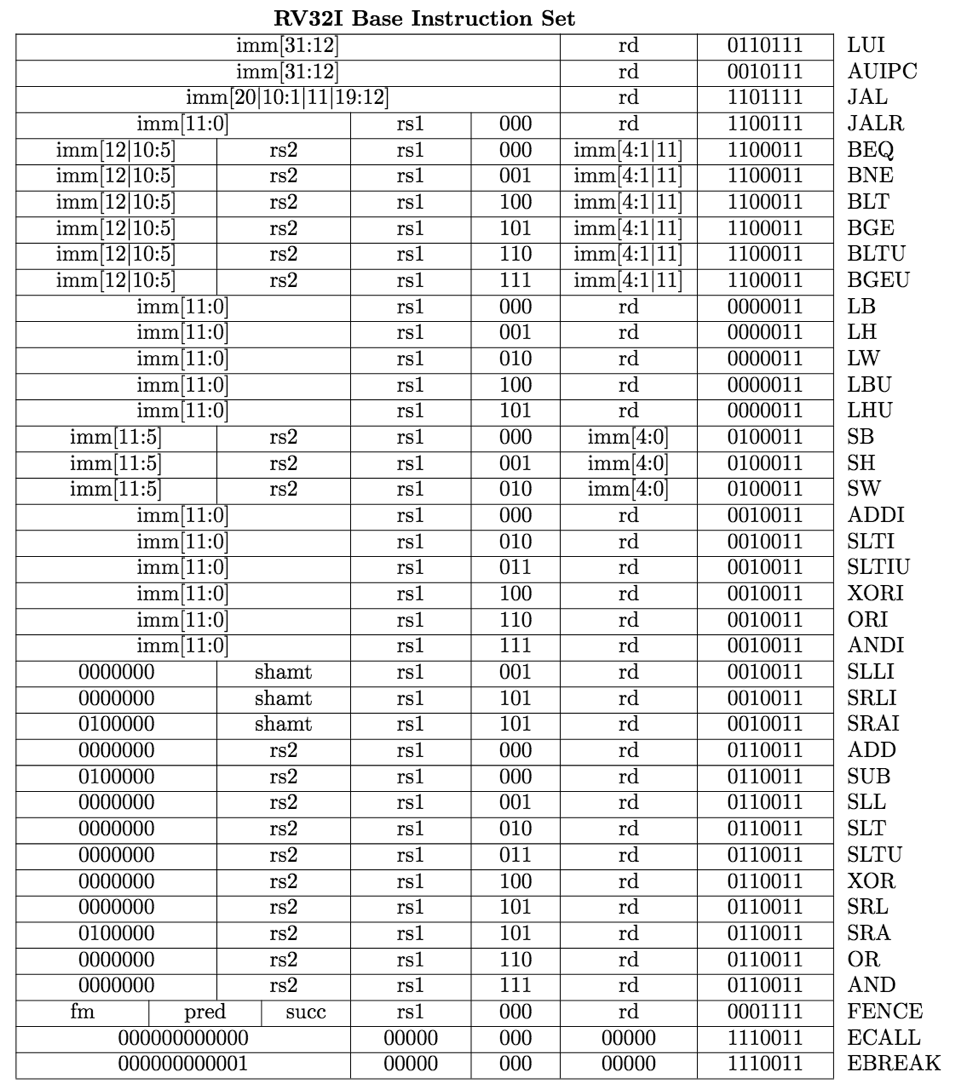
\includegraphics[width=.9\textwidth]{Codage_instructions.png}
\vspace{2ex}
\end{center}

\begin{center}
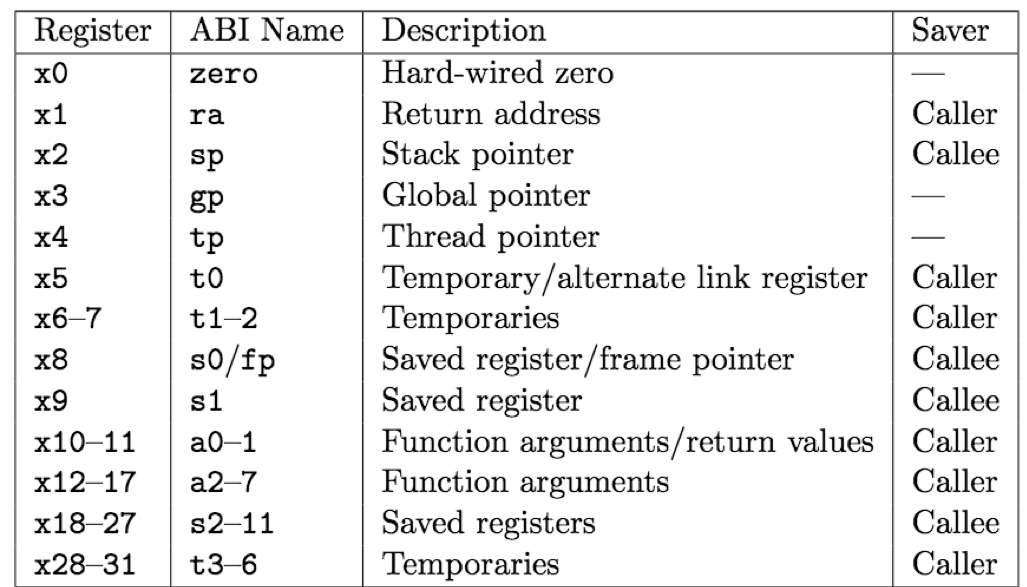
\includegraphics[width=0.7\textwidth]{registres.png}
\vspace{2ex}
\end{center}

\end{document}
